\documentclass{tufte-handout}

\title{A Note on Run Times and Scaling}

\author{David Dobor}

\date{January 29, 2016} % without \date command, current date is supplied

%\geometry{showframe} % display margins for debugging page layout

\usepackage{graphicx} % allow embedded images
  \setkeys{Gin}{width=\linewidth,totalheight=\textheight,keepaspectratio}
  \graphicspath{{graphics/}} % set of paths to search for images
\usepackage{amsmath}  % extended mathematics
\usepackage{booktabs} % book-quality tables
\usepackage{units}    % non-stacked fractions and better unit spacing
\usepackage{multicol} % multiple column layout facilities
\usepackage{lipsum}   % filler text
\usepackage{fancyvrb} % extended verbatim environments
  \fvset{fontsize=\normalsize}% default font size for fancy-verbatim environments

% Standardize command font styles and environments
\newcommand{\doccmd}[1]{\texttt{\textbackslash#1}}% command name -- adds backslash automatically
\newcommand{\docopt}[1]{\ensuremath{\langle}\textrm{\textit{#1}}\ensuremath{\rangle}}% optional command argument
\newcommand{\docarg}[1]{\textrm{\textit{#1}}}% (required) command argument
\newcommand{\docenv}[1]{\textsf{#1}}% environment name
\newcommand{\docpkg}[1]{\texttt{#1}}% package name
\newcommand{\doccls}[1]{\texttt{#1}}% document class name
\newcommand{\docclsopt}[1]{\texttt{#1}}% document class option name
\newenvironment{docspec}{\begin{quote}\noindent}{\end{quote}}% command specification environment


\usepackage{listings}
\usepackage{color}

\definecolor{dkgreen}{rgb}{0,0.6,0}
\definecolor{gray}{rgb}{0.5,0.5,0.5}
\definecolor{mauve}{rgb}{0.58,0,0.82}

\lstset{frame=tb,
  language=matlab,
  aboveskip=3mm,
  belowskip=3mm,
  showstringspaces=false,
  columns=flexible,
  basicstyle={\small\ttfamily},
  numbers=none,
  numberstyle=\tiny\color{gray},
  keywordstyle=\color{blue},
  commentstyle=\color{dkgreen},
  stringstyle=\color{mauve},
  breaklines=true,
  breakatwhitespace=true,
  tabsize=3
}



\begin{document}

\maketitle% this prints the handout title, author, and date

\begin{abstract}
\noindent We argue why a quadratic run-time of an algorithm is much too slow. The reason for this is that 
$O(n^2)$ algorithms do not sclale: as computers get faster and bigger, quadratic time
algorithms actually get slower. We explain here what that means.
\end{abstract}


\section{What's wrong with $O(n^2)$?}

Many of the algrotims we considered so far, like insertion sort or selection sort, had $O(n^2)$ 
worst case running time. Large problems simply can not be solved by procedures
that are this slow.

\bigskip
A rough standard for now is that people have computers that run billions of operations per second and 
have billions of entries in main memory.  For example, I'm typing this on a 2.2 GHz device with 8 GBytes
of main memory.  

\begin{marginfigure}
  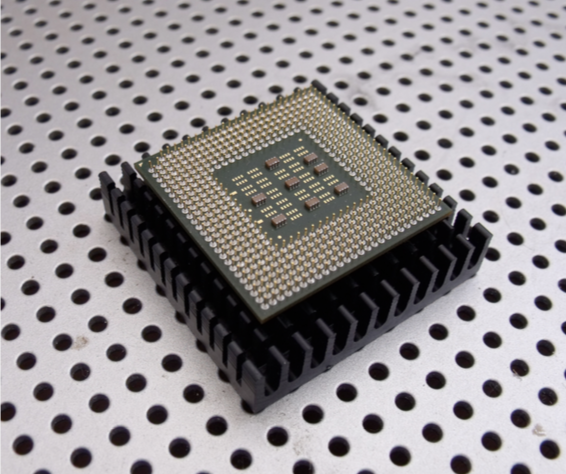
\includegraphics{processor}
  \caption{A modern processor.}
\end{marginfigure}

\bigskip
This means that you can touch everything in main memory on the order of about a second.

\bigskip
It is kind of an amazing fact that this rough stadard has held for longer than over past half-a-century. The 
computers get bigger but they also get faster. To touch everything in memory is going to take a few seconds.
This was true when computers had a few thousand words of memory, and it is true now when they have billions
or more. So let's accept that for a moment as what computers are like.

\bigskip
What that means is that with that huge memory we can address huge problems. So we can have billions of 
objects and hope to sort them using bubble-sort, for example. 

\bigskip
But there is a problem here. A $O(n^2)$ algoritm taking as input $n = 10^9$  entries will perform about 
$(10^9)^2 = 10^{18}$  operations. This, on a computer that processes $10^9$ entries per second, will 
take $10^{18} / 10^9 = 10^9$ seconds.  Well, this works out to be over \emph{30 years of computing time.} 
Obviously, it is not practical to address such a problem on today's computer.  

\newthought{Now consider} a computer that is 10 times as fast on which you can address a problem that is 10 times as big and 
which you will probably get to play with in not so distant future. 

\begin{marginfigure}
  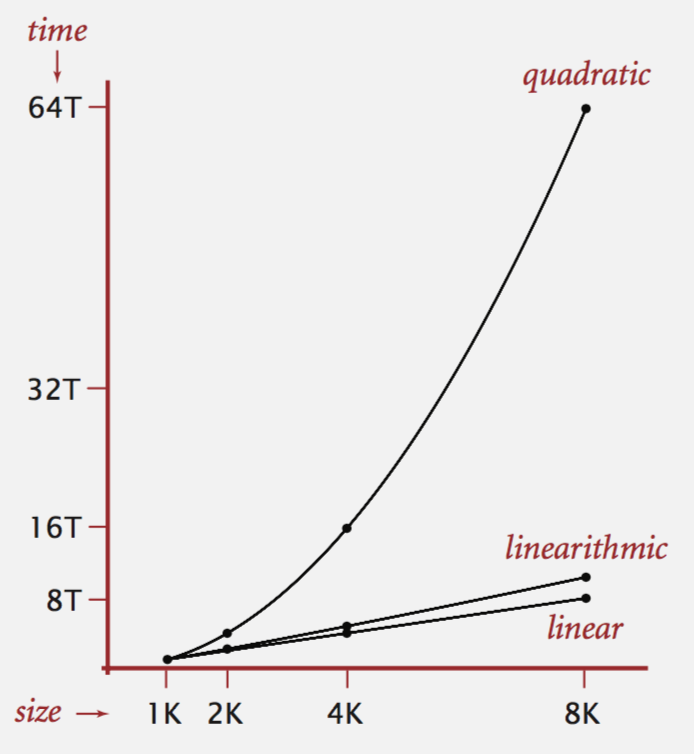
\includegraphics{graph}
  \caption{A $O(n^2)$ algoritm scales horribly.}
\end{marginfigure}

\bigskip
The same algortimg will take (10 billion)$^{2} = (10^{10})^2 = 10^{20}$ operations on a device with with 
$10^{10}$ memory entries, all of which can be accessed in about a second. How long would that take? 
$10^{20} / 10^{10} = 10^{10}$ seconds. Well, this works out to be over \emph{300 years of computing time.} 




This is exactly the kind of situation you would want to try to avoid by developing algoritms that perform better. 



\end{document}




















